Negli ultimi anni si è assistito a un'enorme diffusione di Internet e soprattutto di una varietà di dispositivi con i quali è possibile accedervi: mentre agli albori esistevano solamente PC desktop, con i quali poter visitare pagine per lo più statiche, al giorno d'oggi sono disponibili dispositivi come smartphone e tablet che ci permettono di rimanere sempre connessi. Grazie al fatto di essere estremamente portatili e semplici da utilizzare essi sono ormai diventati oggetti indispensabili nella vita quotidiana. Lo scorso anno è avvenuto il sorpasso della quantità di traffico generata da smartphone e tablet rispetto ai PC (Figura \ref{fig:traffico-tipologia-dispositivo}). L'incremento della velocità delle connessioni e il progresso tecnologico ha fatto sì che sia possibile consultare qualsiasi tipo di informazione su internet, dal semplice testo fino a immagini, video, ecc.

\begin{figure}[ht]
	\centering
	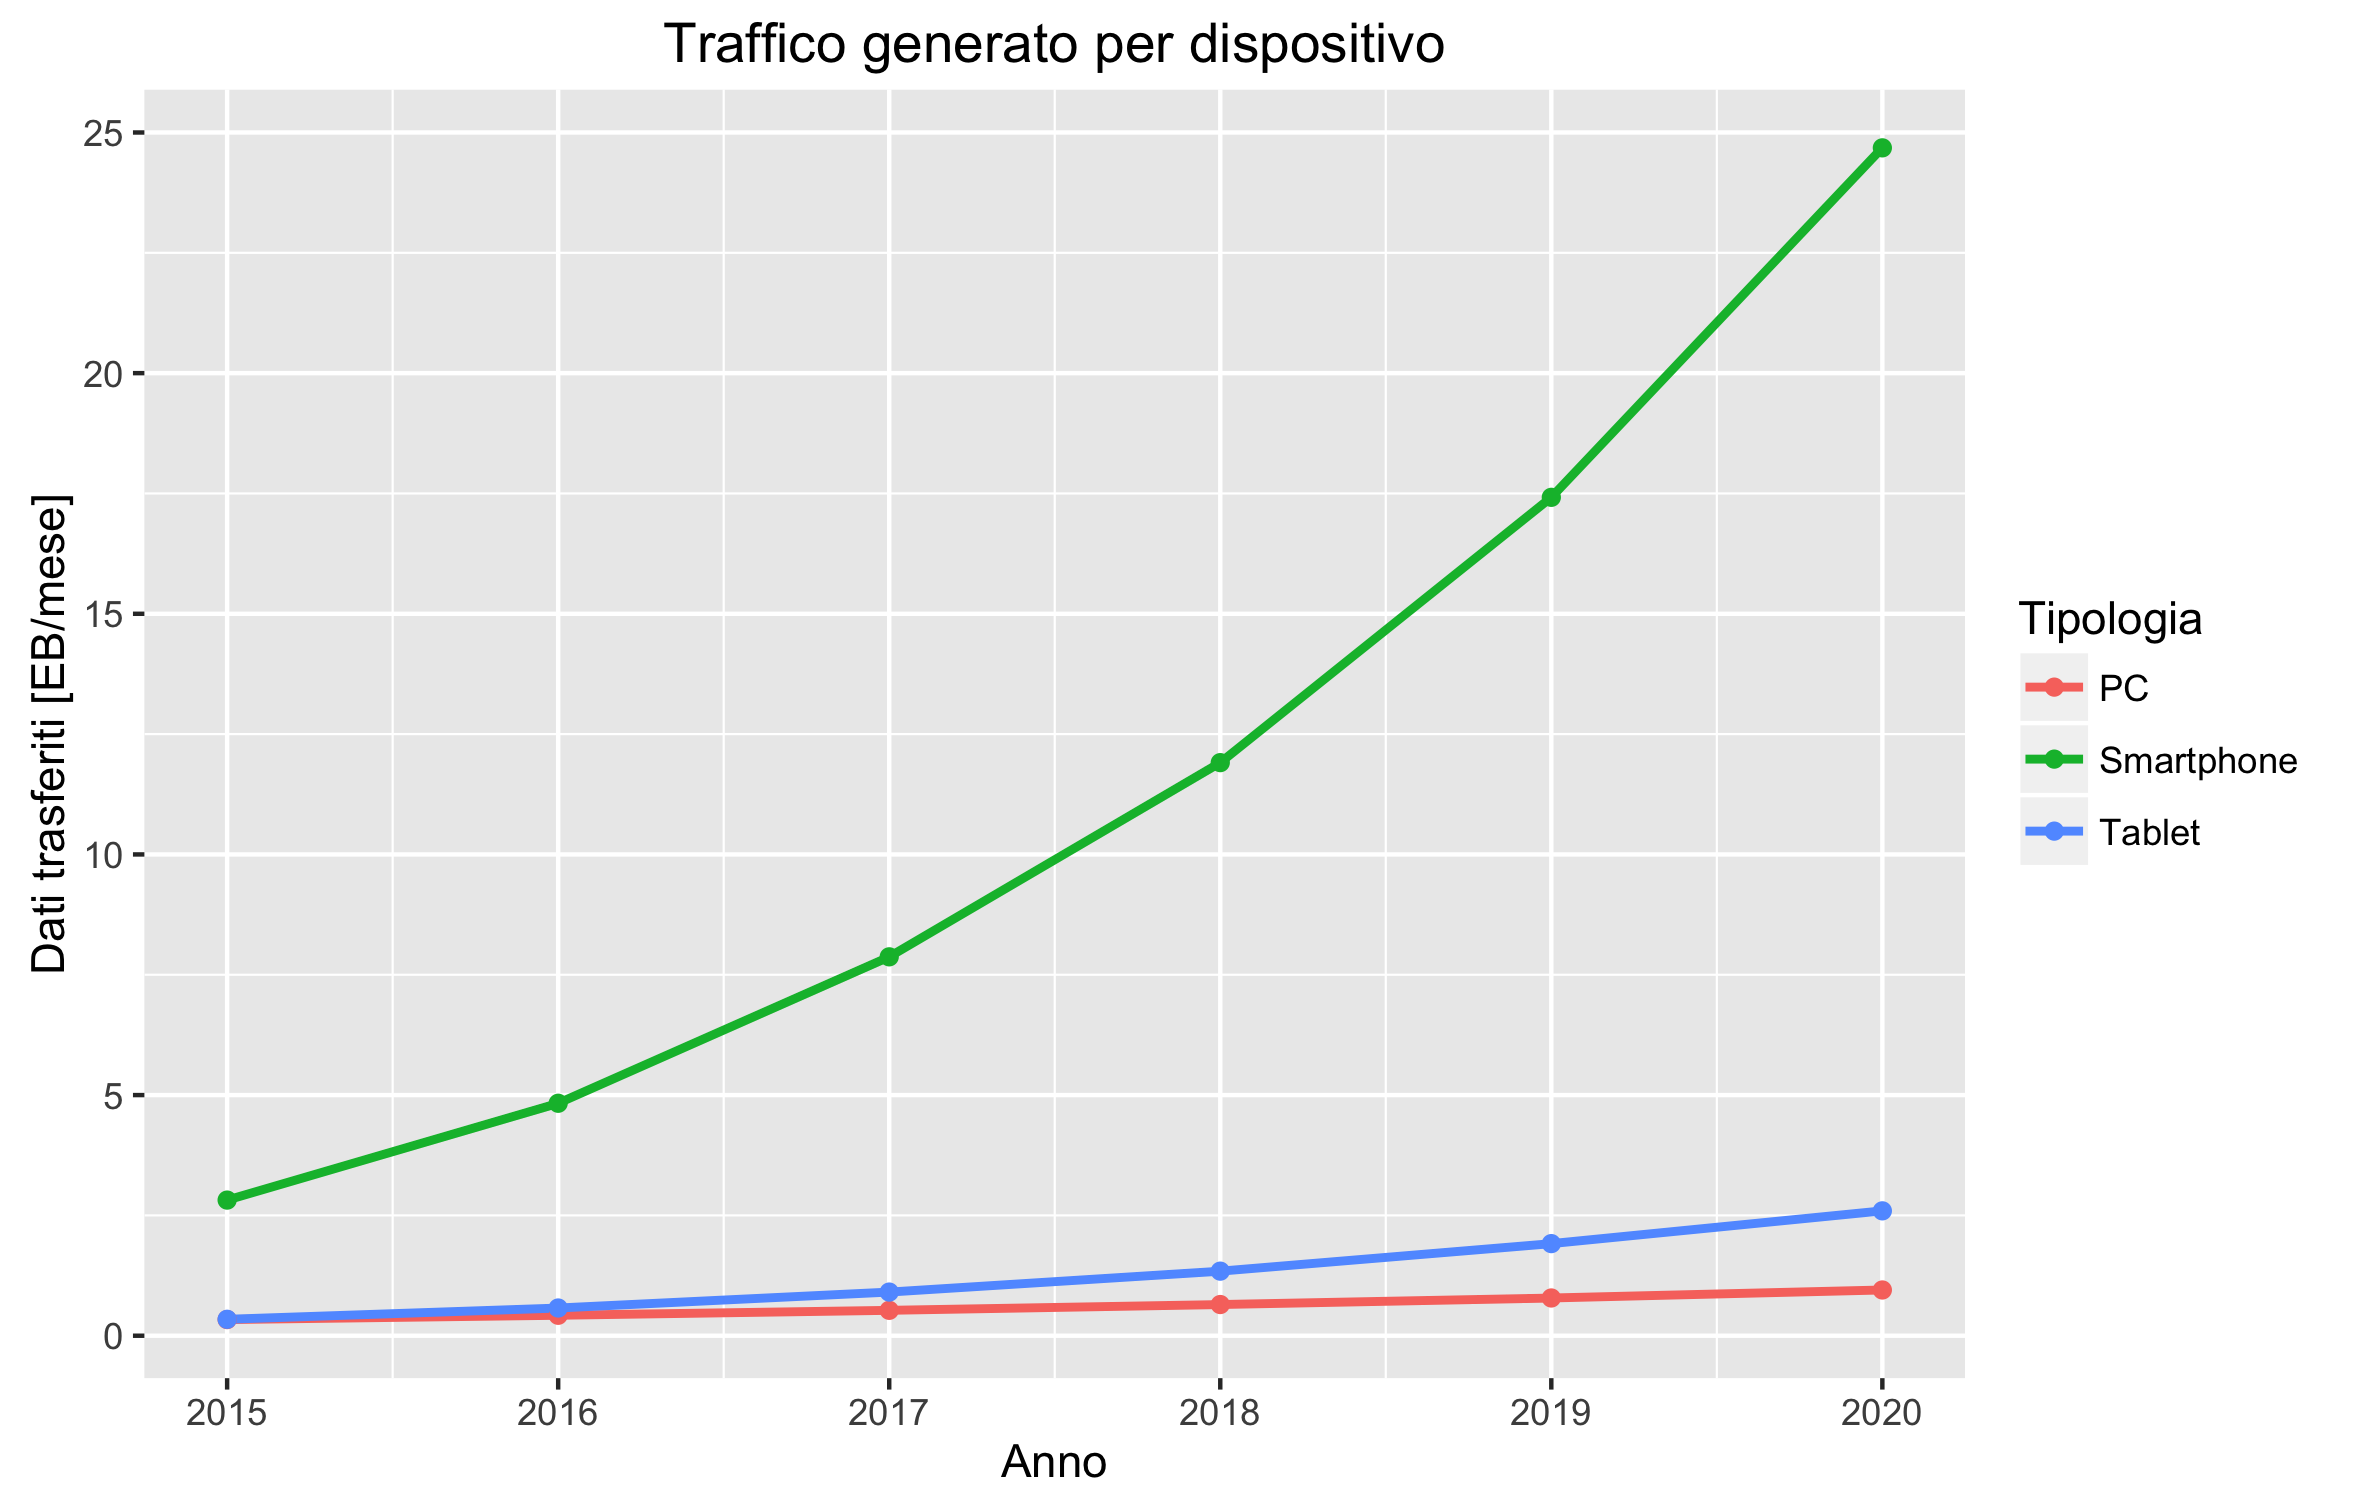
\includegraphics[width=\textwidth]{1-introduzione/Immagini/traffico-dispositivi.png}
	\caption[Traffico generato per tipologia di dispositivo]{Traffico generato per tipologia di dispositivo (fonte: Cisco, 2016)\label{fig:traffico-tipologia-dispositivo}}
\end{figure}

Si è persa anche la tradizione che sia un gestore a pubblicare contenuti in quanto ormai sono direttamente gli utenti a produrre la maggior parte delle informazioni disponibili (Figura \ref{fig:analisi-dati-generati}). Questo fenomeno è stato accentuato con la creazione dei \emph{social network}, che permettono di creare collegamenti tra le persone e dove è possibile condividere qualunque cosa che ognuno trova interessante. Gli utenti vengono così coinvolti nella creazione di contenuti di vario tipo. Per esempio possono essere anche di tipo multimediale, grazie alla dotazione di fotocamera ad alta risoluzione nei dispositivi.

\begin{figure}[ht]
	\centering
	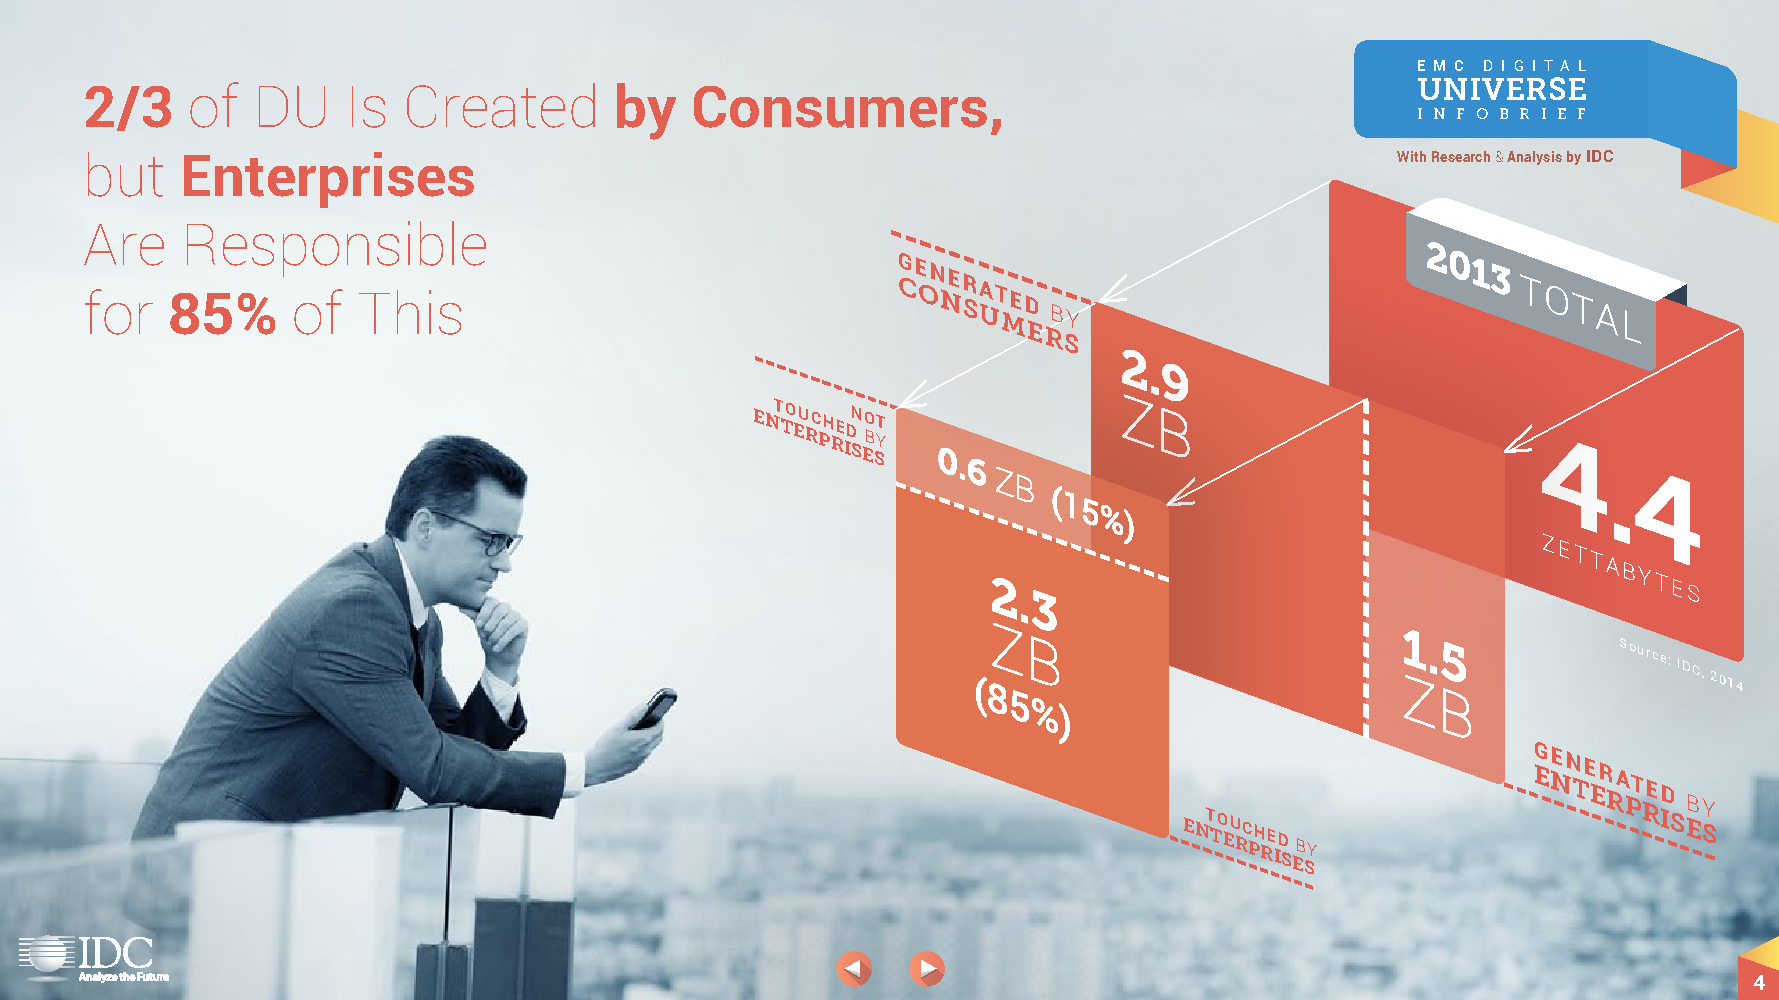
\includegraphics[width=\textwidth]{1-introduzione/Immagini/dati-generati-consumer.pdf}
	\caption[Analisi della quantità di dati generati]{Analisi della quantità di dati generati (fonte: IDC, 2014)\label{fig:analisi-dati-generati}}
\end{figure}

Come si può notare in Figura \ref{fig:traffico-categoria-applicazione} il traffico video e audio è in costante aumento. In particolare il traffico di video sovrasta tutti gli altri, anche a causa della maggior dimensioni di questi contenuti. Questo fenomeno è dovuto anche alla crescita dei servizi che permettono lo \emph{streaming} dei contenuti multimediali come YouTube\footnote{YouTube: \url{https://www.youtube.com}} o Netflix\footnote{Netflix: \url{https://www.netflix.com}}.

\begin{figure}[ht]
	\centering
	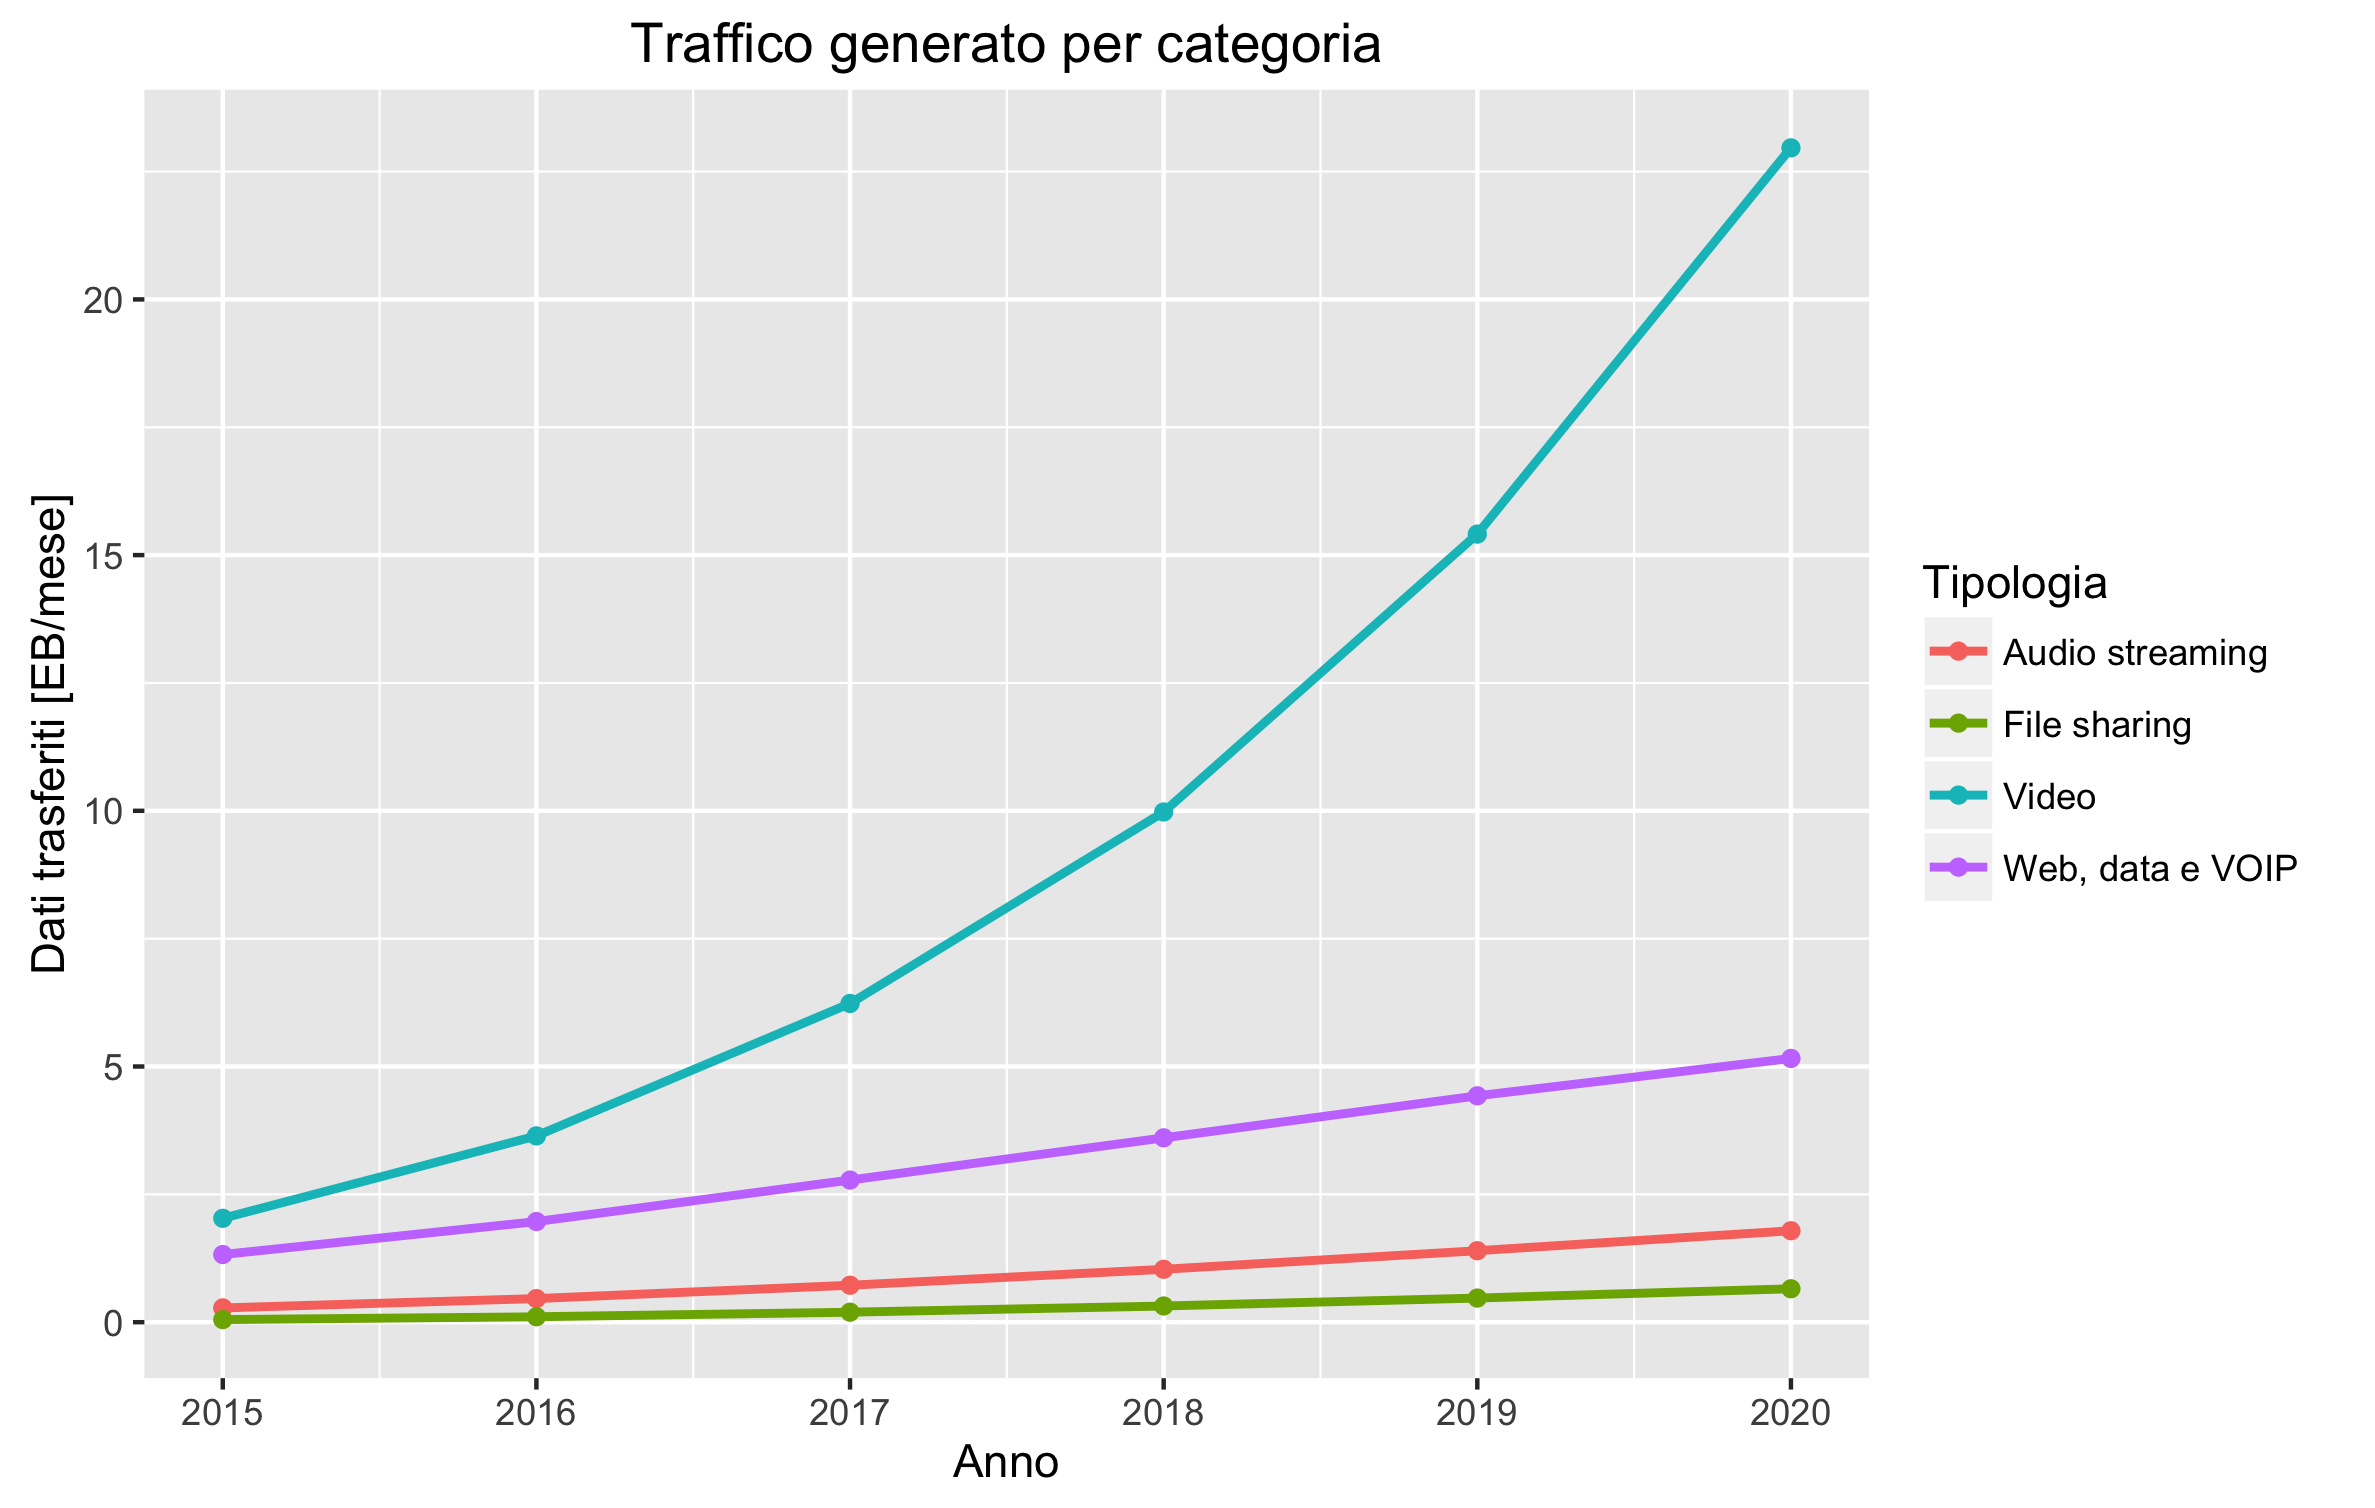
\includegraphics[width=\textwidth]{1-introduzione/Immagini/traffico-categoria.png}
	\caption[Traffico generato per categoria di applicazione]{Traffico generato per categoria di applicazione (fonte: Cisco, 2016)\label{fig:traffico-categoria-applicazione}}
\end{figure}

Internet è diventato una fonte immensa di informazioni, che sono destinate ad aumentare. Un recente trend è relativo ai dispositivi connessi, definito \emph{Internet of Things} (Figura \ref{fig:statistiche-iot}). L'idea è che qualsiasi dispositivo può essere connesso a Internet per generare informazioni, in particolare tutti quelli provvisti di \emph{sensori} che possono fornire dati sullo stato dell'ambiente nel quale si trovano.

\begin{figure}[ht]
	\centering
	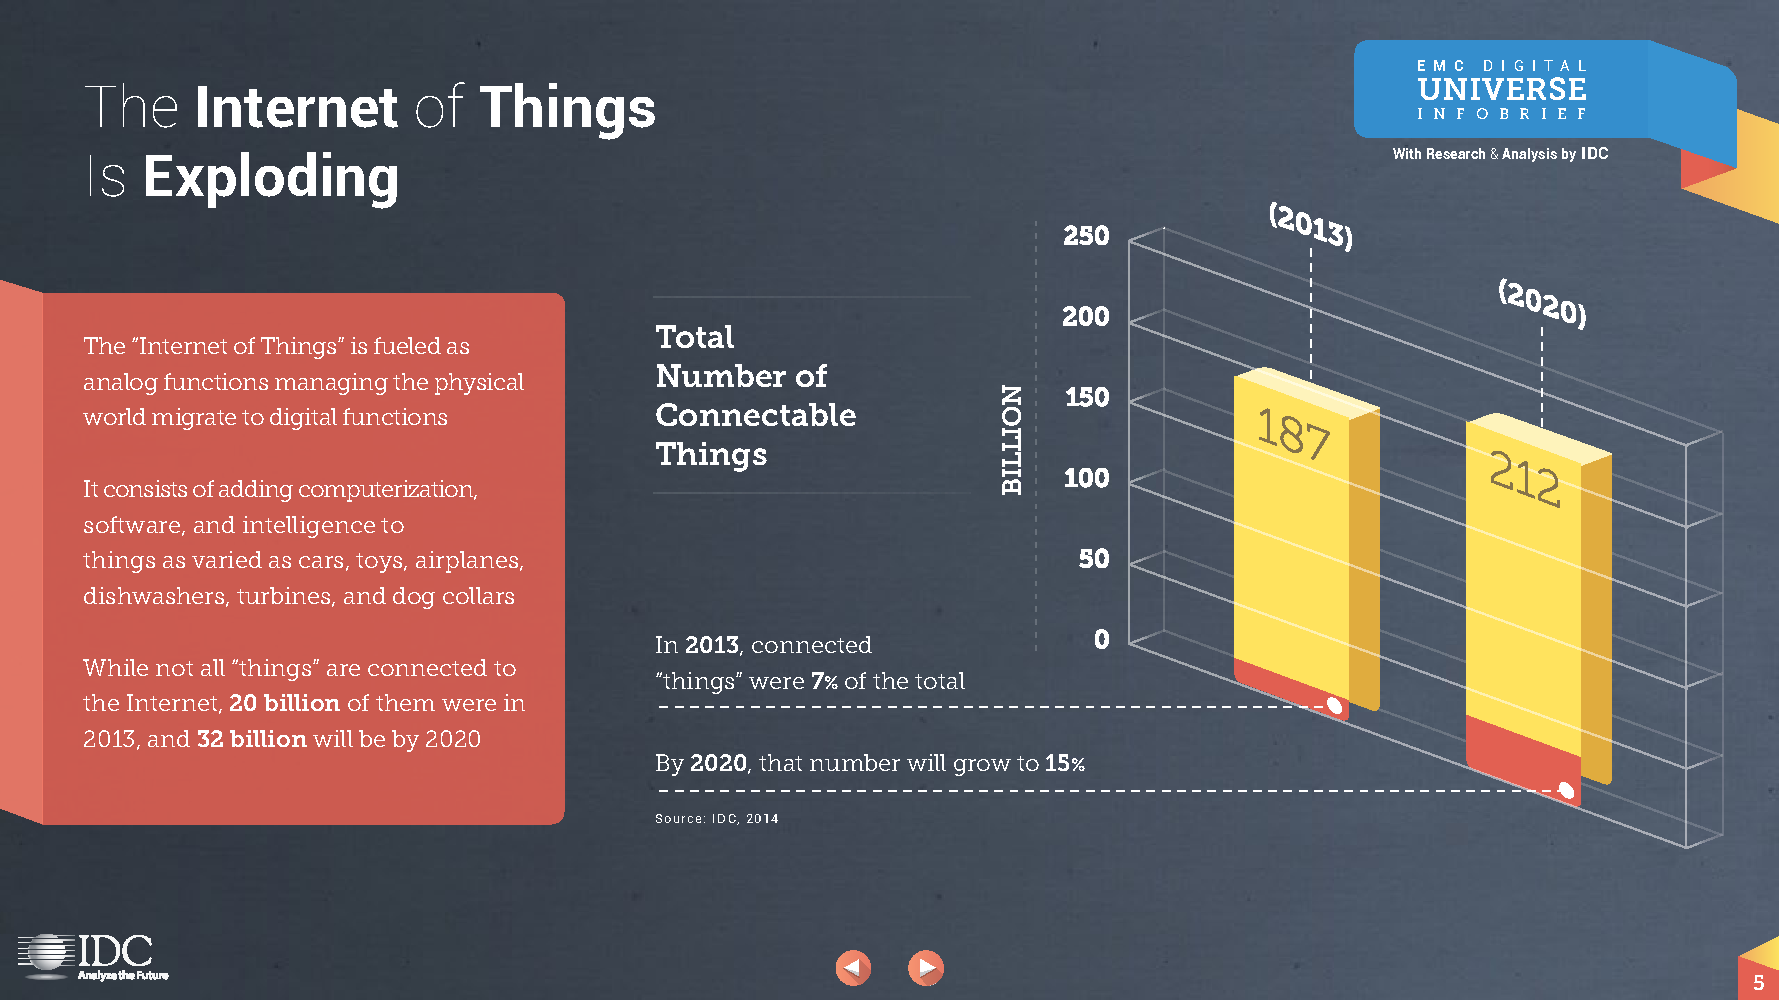
\includegraphics[width=\textwidth]{1-introduzione/Immagini/iot-trend.pdf}
	\caption[Statistiche sull'Internet of Things]{Statistiche sull'Internet of Things (fonte: IDC, 2014)\label{fig:statistiche-iot}}
\end{figure}

%Inizio parte del contesto
Uno dei principali problemi che chiunque lavori coi dati vuole cercare di risolvere è ridurre lo \virgolette{information noise}, migliorando la precisione delle informazioni da mostrare, in maniera che meglio si adattino ai requisiti.

\upe frequente che le informazioni non vengano acquisite unicamente da una base di dati bensì provengono da più fonti, anche di tipologie diverse tra loro (es.: relazionali, XML, ec..). Basti pensare alla moltitudine di servizi presenti nel web.

Questo aumento della quantità di informazioni, se non propriamente controllato, può provocare un ammasso di dati che genera soltanto confusione piuttosto che fornire elementi utili, riducendo i benefici che invece si potrebbero ricavare da tutte queste informazioni. Tuttavia, distinguere le informazioni rilevanti da quelle che non lo sono è un compito tutt'altro che semplice: alcune informazioni potrebbero essere trattate in maniera differente, anche per lo stesso utente, che in diverse situazioni ha bisogno di informazioni differenti. 

Si parla dunque di sistemi \emph{context aware}, che si occupano dell'\emph{acquisizione} del contesto (per esempio tramite l'utilizzo di determinati sensori), l'\emph{astrazione} e il \emph{riconoscimento} del contesto (per esempio associare un determinato stimolo al contesto) e il \emph{comportamento} adatto alla situazione riconosciuta (per esempio l'esecuzione di un'azione innescata dal contesto) \cite{schmidt2003ubiquitous}. L'utilizzo del \emph{contesto} permette la realizzazione di interfacce grafiche innovative e viene spesso utilizzato nella \emph{computazione ubiqua} e nei \emph{dispositivi indossabili}.

%Resta aperto il problema di come visualizzare le operazioni e come ricercare le info in modo semplice (Fornire interfaccia per permettere agli utenti di cercare le informazioni)

Una volta acquisite le informazioni nasce l'esigenza di definire regole su come mostrarle all'utente finale. Con la diffusione di dispositivi mobili sempre più sofisticati si è resa maggiormente necessaria un'esperienza utente semplice che lo guidi durante le sue attività .

%	parlare di come sia conveniente un meccanismo decori le informazioni testuali con contenuti aggiuntivi, come mappe, foto e altre cose dinamiche}

Per questo motivo ha assunto un ruolo di grande importanza l'esperienza d'uso dell'utente (\emph{User Experience}). Infatti se un'applicazione non è ben formata e non è fruibile in modo semplice dall'utente, il numero di utenti che la utilizzeranno calerà sempre di più. Secondo Gary Illyes di Google \virgolette{circa il 61 percento degli utenti che incontrano problemi con siti e app su smartphone ne abbandonano l'utilizzo volontariamente}\footnote{Search Engine Land Interview to Gary Illyes of Google: \url{http://searchengineland.com/google-may-add-mobile-user-experience-ranking-algorithm-205382}}. Per evitare questo problema è necessario prestare un'attenzione sempre maggiore a come viene progettato tutto il flusso di navigazione dell'utente e a fornirgli i dati necessari per poter sfruttare al meglio l'applicazione. L'aggiunta di elementi comprensibili in modo intuitivo come mappe e foto porta l'utente a utilizzare altre aree della mente, come quella della memoria fotografica. In questo modo l'utente può facilmente acquisire conoscenza utilizzando diversi dati e diverse tipologie di visualizzazione.

%inizio parte di progetto

\upe proprio per cercare nuovi strumenti in grado di migliorare l'esperienza dell'u\-ten\-te nell'esplorazione delle informazioni che nasce il progetto CAMUS. CAMUS è l'a\-cro\-ni\-mo di \virgolette{Context Aware Mobile mashUpS}. CAMUS permette la creazione di applicazioni dinamiche che integrano dati provenienti da fonti differenti ed adattandoli alle esigenze dell'utente. Partendo dalla sigla si possono intuire le due anime principali che sono alla base del progetto: il \emph{contesto} e i \emph{mashup}.

Per quanto riguarda l'aspetto del \emph{contesto}, nella tesi si andrà ad affrontare la modellazione della situazione. \upe un'attività molto delicata, in quanto esistono una moltitudine di parametri che possono definire un particolare momento. \upe necessario fare un scelta di quali siano gli indicatori più idonei e quali invece possono essere scartati. L'obiettivo è fornire un modello che permetta di definire in maniera adeguata il contesto nel quale si trova l'utente che sia \emph{semplice}: non si potranno utilizzare formalismi complessi che creino problemi nell'utilizzo altrimenti si andrebbe in contrasto coi principi di \emph{User Experience} precedentemente citati.

Per la tematica dei \emph{mashup} viene preso in considerazione l'aspetto di acquisire le informazioni da più fonti di diverso tipo. CAMUS prevede un sistema flessibile che gli permetta di acquisire informazioni da diverse fonti, andando così ad aumentare il potere conoscitivo che si può fornire all'utente. Come detto in precedenza bisogna però stare particolarmente attenti all'utilizzo di grosse quantità di dati, in quanto se non opportunamente trattate e filtrate possono generare solamente confusione e risultare così inutilizzabili per l'utente. Nasce così l'intuizione di utilizzare il contesto come metodo di selezione dei dati che sono più rilevanti per l'utente. Il contesto mette a disposizione lo stato in cui si trova l'utente, le condizioni dell'ambiente che lo circonda e i suoi interessi personali. Si ritiene che queste preziose informazioni possano essere uno strumento determinante per mettere ordine ai dati e fornire così solo le informazioni che sono interessanti per l'utente in quel dato momento. In questo modo è possibile sfruttare tutte i dati che si hanno a disposizione senza il rischio di sovraccaricare l'utente con informazioni non necessarie.

CAMUS si propone quindi come un \emph{framework} per permettere la realizzazione di app mobili che si adattino sia alle preferenze dell'utente sia alla situazione nella quale si trova. L'idea è che l'utilizzo di modelli per definire il contesto e per schematizzare la composizione dell'interfaccia grafica possano portare enormi benefici nell'interazione tra utente e applicazione. Viene permessa un'elevata \emph{personalizzazione} dell'applicazione, sia per quanto riguarda i contenuti sia per l'aspetto col quale si presenta. %Si vuole mettere l'utente al centro del processo e gli strumenti che utilizza per cercare informazioni devono lavorare per lui e quindi adattarsi alle sue esigenze e necessità.
Si vuole avere una rappresentazione dei contenuti che rappresenti la tipologia di informazione in maniera ottimale. Inoltre si vuole sfruttare la multimedialità messa a disposizione dei recenti dispositivi mobili per coinvolgere maggiormente l'utente e semplificargli il compito.

Certamente il problema principale riguarda l'organizzazione fisica delle informazioni. Visto che CAMUS non viene limitato ad uno specifico contesto, è necessario prevedere un meccanismo che permetta di adattare la visualizzazione di categorie diverse di informazioni. Come è facilmente intuibile mostrare un elenco di film è ben diverso da mostrare un elenco di ristoranti. Un primo punto da snodare è quindi relativo alla creazione di uno schema flessibile che permetta di descrivere come visualizzare queste informazioni sul dispositivo.

Ma non solo: questo schema deve essere anche in grado di raccogliere informazioni di contorno che permettano di migliorare l'esplorazione di queste informazioni. Per esempio, se si sta cercando un ristorante può essere d'aiuto avere a disposizione una galleria di foto del locale con i piatti che offre, di una mappa che indichi dove si trova il ristorante o delle informazioni sul meteo, per decidere se prenotare all'esterno o all'interno. Invece se si sta cercando un film può essere sicuramente d'aiuto avere un trailer da vedere per farsi un'idea del film oppure l'elenco dei cinema che l'hanno in programmazione.

Quelle descritte sono operazioni non sempre alla portata degli utenti, soprattutto per quanto riguarda la modellazione del contesto o la composizione dell'interfaccia grafica. Quando il contesto diventa in grado di descrivere diverse realtà assume anche dimensioni notevoli. Avere troppe scelte a disposizione rende vani gli sforzi per cercare di mettere ordine nei dati, in quanto verrebbe solamente spostato il problema a un altro livello. Inoltre l'utente non conosce a fondo la struttura dei dati e non può quindi comporre al meglio un'interfaccia completa dei servizi ausiliari che possano migliorare l'esplorazione delle informazioni. Per agevolare l'utente in queste situazioni si è deciso di dare importanza alla figura dell'\emph{esperto di settore}. L'esperto di settore è colui che conosce a fondo l'ambito di utilizzo di una CAMUS app. Si ritiene che questa sua conoscenza permetta di guidare l'utente nelle sue scelte. Uno dei suoi compiti sarà quello di definire insieme all'utente un suo profilo, in base alle sue esigenze, in modo che dal contesto possano essere eliminati i rami non necessari. Inoltre si occuperà di comporre delle interfacce funzionali sia per la situazione sia per l'utente. In questo modo è possibile avere una varietà di composizioni adatte ai diversi ambiti di utilizzo che si adattino anche alle preferenze dell'utente e ad altri fattori, come la località. 
Purtroppo l'esperto di settore non può svolgere tutti i compiti richiesti per il sistema CAMUS, in particolare quelli che richiedono delle competenze informatiche, come per esempio la registrazione di nuovi servizi da utilizzare nella fase di composizione dell'albero di contesto. Per questo motivo si è scelto di introdurre la figura dell'\emph{amministratore}, con il compito di svolgere le funzioni prettamente informatiche. Oltre alla registrazione dei servizi, con tutte le configurazioni delle traduzioni dei termini da quelli utilizzati nei servizi a quelli presenti in CAMUS, l'amministratore deve mantenere aggiornate le tipologie di componenti disponibili nell'applicazione con quelli delle \emph{web app}.

\section{Caso di studio: il turismo\label{sec:caso-studio-turismo}}

In questa sezione viene introdotto un caso di studio, che serve per validare il modello proposto per CAMUS. Utilizzare un esempio di applicazione del framework a un caso reale può essere un utile indicatore al fine di supportare le scelte effettuate e di osservare se sono presenti alcune lacune nella modellazione.

CAMUS ha come obiettivo quello di essere universale, cioè utilizzabile in ambiti anche molto diversi tra loro. Come caso di studio è stato dunque necessario pensare a un ambito che consentisse di sfruttare al meglio le capacità di adattarsi alle varie situazioni nelle quali si può trovare l'utilizzatore dell'app.

\upe stato scelto il caso di studio relativo al settore \emph{turistico}, proprio per via della sua dinamicità. In particolare si è preso in considerazione il caso di un'agenzia di viaggi che deve proporre ai propri clienti dei pacchetti di viaggio.

L'ambito turistico calza a pennello per gli intenti di CAMUS; un viaggio incomincia dalla sua pianificazione: prima di partire, il turista si informa sulla destinazione, quali hotel sono disponibili, con quali mezzi di trasporto è più conveniente raggiungere la destinazione, ecc. In questo frangente CAMUS si propone come \virgolette{suggeritore} di esperienze di viaggio: permette all'utente di non concentrarsi sul \emph{dove} vuole andare, ma sul \emph{cosa} vuole fare. Gli viene data la possibilità di scegliere l'esperienza di viaggio che vuole intraprendere e proporgli così i pacchetti che corrispondono alle sue scelte.

Le potenzialità di CAMUS non terminano una volta che il viaggiatore sceglie la sua meta: l'app gli servirà \emph{durante} il viaggio per informarsi sulle attività da svolgere, le escursioni disponibili, i ristoranti nei quali cenare, ecc. Per esempio, se un utente vuole provare un ristorante tipico della zona, gli basterà aprire l'app CAMUS e selezionare che è interessato nella ricerca dei ristoranti che propongono dei menù \emph{tipici} del luogo. Gli verrà mostrato un elenco dei ristoranti che si trovano nei suoi paraggi che rispettano i criteri definiti. Inoltre gli verranno fornite indicazioni su come raggiungere il ristorante, sfruttando, se specificato nella richiesta, i mezzi pubblici presenti nella destinazione scelta.

Le due figure principali in questo caso di studio sono due: l'\emph{agente di viaggio} e il \emph{turista}. L'\emph{agente} ha il compito di organizzare tutto il viaggio, gestire quindi le prenotazioni, gli spostamenti principali e i soggiorni per il viaggiatore, mentre il \emph{turista} è colui che fisicamente compie il viaggio, che può essere quindi considerato come l'utente finale.

All'agente vengono inoltre demandati i compiti di personalizzazione dell'app: questa fase avviene quando il cliente si presenta nell'agenzia di viaggio. A quest'ultimo vengono prima di tutto fatte alcune domande per conoscere il suo profilo, in modo da adattare le scelte che gli verranno mostrate dall'app. In questo modo è possibile evitare che al cliente vengano proposte troppe scelte che non siano di suo interesse. Inoltre vengono fissate alcune opzioni che tendono a non cambiare nel corso del viaggio; per esempio se l'utente viaggia con un animale domestico questa scelta sarà sempre la stessa durante tutto il viaggio e non gli verrà chiesta di nuovo.%\footnote{CAMUS si schiera contro l'abbandono degli animali: \url{http://www.emergenza24.org/salvaunamico/}}

L'ulteriore compito che può svolgere l'agente è quello di personalizzare l'aspetto grafico dell'app qualora ritenga che sia necessario. Con CAMUS vengono proposti alcuni template predefiniti per ogni categoria e viene lasciata libera scelta all'agente se utilizzarli così come sono o modificarli. Una delle motivazioni nella scelta di modificare l'aspetto riguarda l'aggiunta di alcuni servizi di supporto. Per esempio, se l'agente è consapevole che nel luogo in cui vuole andare il cliente le condizioni meteorologiche sono molto variabili e nella versione predefinita dell'app non sono presenti informazioni meteo, può aggiungere questa indicazione in modo da fornire al turista un'informazione in più per gestire al meglio la sua vacanza.

Come si può notare da questo breve esempio, l'utilizzo di CAMUS in un'agenzia viaggi permette di fornire un servizio più coinvolgente ai propri clienti. La realizzazione di app personalizzate appositamente per un turista permette di effettuare scelte migliori e di proprio interesse. Inoltre estende la capacità dell'agenzia di fornire un'assistenza al proprio cliente anche durante il viaggio: si può affermare che un'app CAMUS assume il ruolo di \emph{assistente di viaggio} e guida il turista durante tutte le fasi della sua esperienza di viaggio.

\section{Struttura della tesi}

Viene ora fornita una panoramica sulla struttura di questa tesi:

\begin{itemize}
	\item 
	Nel Capitolo \ref{ch:nozioni-preliminari}, dopo aver introdotto i modelli e le tecnologie che saranno utilizzate nel resto della tesi, si discute la letteratura sull'argomento
	\item 
	Nel Capitolo \ref{ch:camus} si entra nei dettagli del progetto CAMUS andando a fornire un contesto più ampio di quello appena descritto e mettendo in risalto gli obiettivi che si vogliono raggiungere
	\item 
	Nel Capitolo \ref{ch:metodologia} vengono analizzate nel dettaglio le logiche alla base del framework
	\item 
	Nei Capitoli \ref{ch:implementazione-backend} e \ref{ch:implementazione-app} viene analizzata nel dettaglio l'implementazione rispettivamente lato backend e mobile app. Si analizza l'architettura utilizzata e le scelte tecnologiche che hanno portato alla realizzazione del prototipo
	\item 
	Nel Capitolo \ref{ch:performance} si andranno ad analizzare le prestazioni della soluzione implementata, simulando alcuni casi d'uso simili alle condizioni di regime della piattaforma
	\item 
	Nel Capitolo \ref{ch:conclusioni} si discuteranno le conclusioni del lavoro relativo al progetto e alcuni spunti per futuri miglioramenti al framework
\end{itemize}